\hsection{Inheritance}%
\label{sec:inheritance}%
%
Inheritance or subclassing is one of the most important concepts of \glsFull{OOP}.
A subclass can be derived from one existing class.
It will inherit all the methods and attributes of that class.
It can add new methods and attributes.
It also can overwrite methods, i.e., replace them with other code.
This mechanism of inheritance can be viewed from several different angles.%
%
\begin{sloppypar}%
For example, we could look at this from the perspective of set theory.
We can consider a class as a set of all objects that belong to that class.
Subclasses are then subsets of these sets.
Remember the tree illustration \cref{fig:pythonExceptions} of built-in \pythonil{Exception}-types back in \cref{sec:builtInExceptions}.
The root was formed by \pythonilIdx{BaseException}.
All exception objects instances of this class.
It has a subclass \pythonilIdx{Exception}.
All instances of \pythonilIdx{Exception} are \pythonilsIdx{BaseException}, but not all \pythonilsIdx{BaseException} are \pythonilsIdx{Exception}.
\pythonilIdx{ArithmeticError} is a subclass of \pythonilIdx{Exception}, meaning that all \pythonilsIdx{ArithmeticError} are \pythonilsIdx{Exception}~(but not vice versa).
In this sense, one could say that if a class \pythonil{ClassA} is a subclass of a class \pythonil{ClassB}, i.e., if \pythonil{issubclass(ClassA, ClassB)}\pythonIdx{issubclass}, then \pythonil{ClassA} is also a subset of \pythonil{ClassB}.%
\end{sloppypar}%
%
\begin{equation}%
\pythonil{ClassA} \subseteq \pythonil{ClassB} \Leftrightarrow \pythonil{issubclass(ClassA, ClassB)}\pythonIdx{issubclass}%
\end{equation}%
%
Another perspective is the concept of specialization.
In a reasonable design, subclasses are not just some random or unstructured subsets of their base classes.
Usually, but they describe specific features that all of their instances have and the others not.
If \pythonil{Animal} was a class, then \pythonil{Bird} would be a subclass.
But it would not just be a random group of animals.
It would represent the animals that add special traits such as two feet, wings, feathers, and laying eggs to their animal character.
It could inherit the attribute \pythonil{weight} and the method \pythonil{eat()} from its base class \pythonil{Animal}.
It could have the methods \pythonil{walk()} and \pythonil{fly()}.
\pythonil{Sparrow} and \pythonil{Ostrich} would be special cases, i.e., subclasses, of \pythonil{Bird}, each having peculiar special traits distinguishing from other \pythonils{Bird}.
\pythonil{Ostrich} could overwrite \pythonil{fly()} to raise a \pythonil{NotImplementedError}, for example.

The concepts of inheritance and overwriting of methods makes classes particularly suitable to define and implement \pglspl{API}.
They allow us to create a base class with methods meant for particular tasks.
But we would define the methods as empty hulls, without implementing them.
These methods, in the base class, could do nothing or raise a \pythonil{NotImplementedError}.
They would just define the \pgls{API}.
Subclasses then can implement the methods with meaningful behavior.
Differenz subclasses could implement the \pgls{API} differently.
We could, for example, imagine an \pgls{API} for rendering of documents, which could be implemented in one subclass to produce \pgls{formatPDF} output and in another subclass to produce \pgls{SVG} output.
A user of the \pgls{API} then only needs to understand the documentation and \pglspl{signature} of the methods in the base class.
They can then use any subclass, depending on what output they want.%
%
\hsection{A Hierarchy of Geometric Objects}%
%
\begin{figure}[tb]%
\centering%
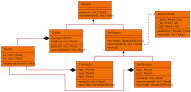
\includegraphics[width=0.985\linewidth]{\currentDir/exampleInheritance}%
\caption{An example for class inheritance. %
The base class \pythonil{Shape} offers two abstract methods, \pythonil{area} and \pythonil{perimeter}. %
The class \pythonil{Circle} inherits from \pythonil{Shape} and implements these methods. %
It also has an attribute \pythonil{center}, which is an instance of~\pythonil{Point}, and an attribute~\pythonil{radius}. %
The class \pythonil{Polygon} extends \pythonil{Shape} as well, and offers, amongst others, an \pythonilIdx{Iterable} of its~\pythonils{Point}. %
It also uses our \pythonil{KahanSum} to implement the \pythonil{perimeter} method. %
The class \pythonil{Polygon} is realized by the classes \pythonil{Triangle} and \pythonil{Rectangle}.}%
\label{fig:exampleInheritance}%
\end{figure}%
%
\gitLoadPython{classes:shape}{}{classes/shape.py}{}%
\listingPython{classes:shape}{%
A class for representing shapes in the two-dimensional Euclidean plane.}%
%
\gitLoadPython{classes:circle}{}{classes/circle.py}{}%
\listingPython{classes:circle}{%
A circle is a special shape, namely the set of all points whose distance from the center of the circle is exactly the radius.}%
%
\gitLoadAndExecPython{classes:circle_user}{}{classes}{circle_user.py}{}%
\listingPythonAndOutput{classes:circle_user}{%
An example of using our class \pythonil{Circle} from \cref{lst:classes:circle}.}{}%
%
\gitLoadPython{classes:polygon}{}{classes/polygon.py}{}%
\listingPython{classes:polygon}{%
Polygons are special shapes delimited by straight lines between corner points.}%
%
\gitLoadPython{classes:rectangle}{}{classes/rectangle.py}{}%
\listingPython{classes:rectangle}{%
Two different points in a plane span a rectangle, which is a special polygon.}%
%
\gitLoadPython{classes:triangle}{}{classes/triangle.py}{}%
\listingPython{classes:triangle}{%
A triangle is a polygon spanned by three points in a plane.}%
%
%
We already learned that classes are a proper tool for grouping data and operations on the data together into one semantic unit.
Classes offer the concept of inheritance, which basically enables specialization.

Imagine that we would wanted to represent all closed geometrical shapes in a two-dimensional Euclidean plane.
The overall structure of this example illustrated in \cref{fig:exampleInheritance}.

We could begin by creating a base class\pythonIdx{class} \pythonil{Shape}.
Each closed shape has an associated \emph{area} as well as a \emph{perimeter}.
Therefore \pythonil{Shape} defines two methods, \pythonil{area} and \pythonil{perimeter}, returning the area in area units and the perimeter length in length units, respectively.
It will not implement them yet, though, because how to compute area and perimeter is different for different types of shapes.
But by defining the methods, we make clear that these two things can be computed for any actual instance of \pythonil{Shape}.

In \cref{lst:classes:shape} with file \programUrl{classes:shape}, we create this base class\pythonIdx{class} \pythonil{Shape}.
The class\pythonIdx{class}~\pythonil{Shape} is not intended for being instantiated directly.
Instead, we just want it to be the base class\pythonIdx{class} for the shape types that we learned about in primary school.
It does not have any attribute.
But, as said, this class has two methods, \pythonil{area} and \pythonil{perimeter}.
Of course, we cannot really compute the area or the perimeter of such an abstract object.
So both methods raise\pythonIdx{raise} an \pythonilIdx{NotImplementedError}.
If someone would like to actually instantiate \pythonil{Shape} by doing, say, \pythonil{s = Shape()} and then invoke \pythonil{s.perimeter()}, this would fail.
This behavior is documented with a \pgls{doctest} in the header of the module.
The important thing is that these methods exist.
All non-abstract subclasses must overwrite and implement them properly.
The user thus can query the area and perimeter of any real instance of \pythonil{Shape} in exactly the same way.

A circle is a special two-dimensional shape.
It does have a center as well as a radius.
Knowing these two attributes, we can draw a circle at its correct location and also compute the area and perimeter.
If we wanted to express this in terms of classes, we could define the class\pythonIdx{class} \pythonil{Circle} as a subclass of class~\pythonil{Shape}.
Not all \pythonils{Shape} are \pythonils{Circle}, but each \pythonil{Circle} is a \pythonil{Shape}.
The class \pythonil{Circle} would have two attributes.
The attribute \pythonil{center} could be an instance of our first ever class \pythonil{Point}.
The attribute \pythonil{radius} could be an \pythonil{int} or a \pythonil{float}.
The methods \pythonil{area} and \pythonil{perimeter} could then be implemented appropriately.

While \pythonil{Shape} itself is useless, it allows us to create different specialized subclasses that do implement \pythonil{area} and \pythonil{perimeter}.
The user of these classes could then treat all of these different subclasses in the same way, because all of them support the interface defined by~\pythonil{Shape}.

In file \programUrl{classes:circle} given as \cref{lst:classes:circle}, we define the class\pythonIdx{class}~\pythonil{Circle}.
By writing \pythonil{class Circle(Shape)}\pythonIdx{class}, we declare it as a subclass\pythonIdx{class} of \pythonil{Shape}.
Via its initializer \dunder{init}, we supply two parameters.
The first one is \pythonil{center}, which is an instance of our class \pythonil{Point} from \cref{lst:classes:point}.
Der zweite ist \pythonil{radius}, which can either be an \pythonil{int} or a \pythonil{float}.
The initializer first checks if \pythonil{radius} is a finite and positive number.
Otherwise, it raises\pythonIdx{raise} a \pythonilIdx{ValueError}.
The initializer of the class\pythonIdx{class}~\pythonil{Point} already ensures that both coordinates of \pythonil{point} will be finite, so we do not need to check these.
We thus ensured that we only create valid circles.

We store \pythonil{center} and \pythonil{radius} in two attributes of the same names.
We annotate them with the \pgls{typeHint} \pythonilIdx{Final}, which means that they should not be changed after the object is constructed.
We thus design our class following the \emph{immutable} approach.

We can now implement the method \pythonil{area} to return~$\numberPi\pythonil{radius}^2$.
We set \pythonil{perimeter} to return~$2\numberPi\pythonil{radius}$.
With this, the complete interface defined by the superclass\pythonIdx{class}~\pythonil{Shape} is now filled with meaning.
We also include comprehensive \pglspl{doctest} in our file, to immediately make sure that the methods work as advertised.

In program \programUrl{classes:circle_user} given as \cref{lst:classes:circle_user}, we explore how this new class can be used.
We create the instance \pythonil{circ} of \pythonil{Circle} by providing the \pythonil{point=Point(2, 3)} and \pythonil{radius=4}.
We confirm that these parameters are indeed reflected by the corresponding attributes.

The operator \pythonil{isinstance(a, B)}\pythonIdx{isinstance} checks whether an object~\pythonil{a} is an instance of class~\pythonil{B}.
If yes, it returns \pythonil{True} and otherwise, it returns \pythonil{False}.
We confirm that \pythonil{isinstance(cir, Circle)}\pythonIdx{isinstance} is \pythonil{True}.
It also holds that \pythonil{isinstance(cir, Shape)}\pythonIdx{isinstance}.
Every instance of \pythonil{Circle} is also an instance of \pythonil{Shape}.
Because \pythonil{Circle} is a special case of \pythonil{Shape}.

It also holds that \pythonil{isinstance(cir, object)}.
\pythonilIdx{object} is the ultimate base class of any class in \python~\cite{PSF:P3D:G:O,PSF:P3D:TPSL:BIF:O}.
If you do not provide a base class in the class definition, \pythonilIdx{object} is used.
This is the case for our class \pythonil{Shape} and also for our older classes \pythonil{Point} and \pythonil{KahanSum}.
Any \pythonil{Circle} is there also an \pythonilIdx{object}.

While the operator \pythonilIdx{isinstance} relates objects to classes, the operator \pythonilIdx{issubclass} does the same thing for two classes.
\pythonil{issubclass(A, B)} is \pythonil{True} if class \pythonil{A} is a subclass, i.e., inherits from, class \pythonil{B}.
Therefore, \pythonil{issubclass(Circle, Shape)} is \pythonil{True} whereas \pythonil{issubclass(Shape, Circle)} is \pythonil{False}.
\pythonil{issubclass(Shape, object)} and \pythonil{issubclass(Circle, object)} are also \pythonil{True} by definition.

There are, of course, more shapes than just circles.
Another very general class of shapes are polygons.
Polygons are shapes enclosed by straight lines.
This means that every polygon can be defined by its corner points.
If we design a class for polygons, then we can appreciate this fact by defining a method \pythonil{points()} returning a sequence of these corner points.

\gitLoadAndExecPython{classes:shape_user}{}{classes}{shape_user.py}{}%
\afterpage{\clearpage%
%
\listingPythonAndOutput{classes:shape_user}{%
An example of how all subclasses of class \pythonil{Shape} can be used in exactly the same way via the methods that are defined in \pythonil{Shape}.}{}%
%
}%
%
In file \programUrl{classes:polygon} presented as \cref{lst:classes:polygon}, we define \pythonil{Polygon} as base class for such shapes.
It is a special case of~(and thus inherits from)~\pythonil{Shape}.
\pythonil{Polygon} extends the interface of \pythonil{Shape} by offering the method~\pythonil{points}.
This method returns an \pythonilIdx{Iterable}\pythonIdx{typing.Iterable} of instances of~\pythonil{Point}, which are the corner points of the polygon.
Our goal here is to provide a base class for different types of \pythonils{Polygon}.
We do not actually want to implement a datastructure for arbitrary polygons directly.
So the method \pythonil{points} raises\pythonIdx{raise} an \pythonil{NotImplementedError} and thus must be implemented by the subclasses that we will develop later.

So we assume that non-abstract sublclasses of \pythonil{Polygon} will always implement method \pythonil{points} appropriately, to return the sequence of corner points of the polygon.
If we know the sequence corner points and also know that they are connected by straight lines, then we can easily compute the perimeter of such a shape.
We can thus implement the method \pythonil{perimeter} as follows:
We iterate over the instances of~\pythonil{Point} returned by~\pythonil{points()}.
In a summation variable, we add up the distance between each point and its successor in the sequence.
Finally, we add the distance of the last point to the first point.

The distances can be computed with the \pythonil{distance} method offered by the \pythonil{Point} class.
While \pythonil{Polygon} itself does not implement \pythonil{points}, its subclasses will.
The method \pythonil{perimeter} will then \emph{automatically} use the actual implementation of the subclass.
If we call \pythonil{a.perimeter()}, then the implementation of \pythonil{points()} of the subclass to which \pythonil{a} belongs will be used.
We therefore can implement \pythonil{perimeter} here, even if \pythonil{points} is not yet implemented.
If we create a subclass that does implement \pythonil{points} and call \pythonil{perimeter} upon an instance of this subclass, it will work.

The summation of the distances could be easily done with a normal variable of type~\pythonil{float}.
However, since we implemented the second-order \citeauthor{K1965PFRORTE}-\citeauthor{B1968NSIMA}-\citeauthor{N1974REVZSES} summation algorithm in~\cref{lst:classes:kahan_sum}, we instead use that one.
It should give us a very accurate result.
Notice that we could not easily use~\pythonilIdx{fsum} here without first storing all distances in a list.
The reason is that we need to add up over the sequence of points and \emph{also} the distance from the last to the first point.
So our \pythonil{KahanSum} does have indeed some advantages.

For convenience sake, we also add a method~\pythonil{print} to \pythonil{Polygon}, which just prints the sequence of points.
So we learned that subclasses can also add new methods and behavior.
We also learned that subclasses themselves can be designed to be abstract subclasses.
And we learned that if we call \pythonil{a.method()}~(or \pythonil{self.method()} inside a method), then this will always invoke the \inQuotes{most recent} implementation of \pythonil{method} in the hierarchy of classes to which object~\pythonil{a} belongs.

Rectangles and triangles are special cases of polygons.
We now implement them as classes \pythonil{Rectangle} and \pythonil{Triangle} in \cref{lst:classes:rectangle,lst:classes:triangle}, respectively, which both are subclasses of~\pythonil{Polygon}.

The class \pythonil{Rectangle} for representing rectangles is implemented in file \programUrl{classes:rectangle}.
A rectangle can be defined using its bottom-left and top-right corner point.
The initializer \dunder{init} of the class \pythonil{Rectangle} thus accepts two points~\pythonil{p1} and~\pythonil{p2} as parameters.
We raise\pythonIdx{raise} a \pythonilIdx{ValueError} if these to points are the same and don't actually form a rectangle.
Otherwise, we store the minimum x\nobreakdashes-~and y\nobreakdashes-coordinate in the bottom-left point attribute~\pythonil{p1}.
We store the maximum x\nobreakdashes-~and y\nobreakdashes-coordinate in the attribute~\pythonil{p2}, marking the top-right corner of our rectangle.

We implement the method \pythonil{points} to return all four corners of the rectangle.
We only needed to store two of them, but we here need to return all four to comply with the definition of the method as given in class~\pythonil{Polygon}.
We simply create the points on the fly and return them in a tuple.

The area of the rectangle is easily computed.
The method \pythonil{area} therefore just has to compute the height and width of the rectangle and multiply them with each other.
The width is the difference of the x\nobreakdashes-coordinates of the two corner points.
The height is the difference of the y\nobreakdashes-coordinates of the two corner points.

While we already inherit a perfectly fine method \pythonil{perimeter} computing the perimeter of our rectangle from \pythonil{Polygon} based on the result of \pythonil{points}.
But we still override it.
This makes sense because we can compute the perimeter faster and more exactly by simply returning twice the sum of the width and height of the rectangle.
The inherited \pythonil{perimeter} method would instead iterate over all four points and compute Euclidean distances using~\pythonil{sqrt}.
This is both slower and less accurate, especially if our coordinates would be~\pythonils{int}.

The class \pythonil{Triangle} for representing triangles is implemented in file \programUrl{classes:triangle}.
This time, we need to store all three corner points.
Of course, in the initializer \dunder{init}, we first check if any side has a zero length, which would mean that the points do not describe a valid triangle.
We raise an \pythonilIdx{ValueError} if so.

We return all three points in the \pythonil{points}~method implementation.
There is no better way for computing the perimeter than what \pythonil{Polygon} already provides, so we this time do not override~\pythonil{perimeter}.
The area computation is implemented using the formula~$A=x_1(y_2-y_3)+x_2(y_3-y_1)+x_3(y_1-y_2)$ that you may remember from school maths.

Notice that both subclasses of \pythonil{Polygon} offer some \pglspl{doctest} in the \pglspl{docstring}.
While I needed to keep the \pglspl{docstring} short to be able to fit the listings on pages, these \pglspl{doctest} still are instructive for the user.

In program \programUrl{classes:shape_user} illustrated as \cref{lst:classes:shape_user}, we now use all the classes derived from \pythonil{Shape}.
All of them support the methods \pythonil{area} and \pythonil{permeter}.

We declare a variable \pythonil{shapes} to hold a list of one instance for each of these subclasses.
We can annotate the list with the \pgls{typeHint} \pythonil{list[Shape]}.
This \pgls{typeHint} states that the list can only include instances of type \pythonil{Shape}.
Since all instances of \pythonil{Circle}, \pythonil{Rectangle}, or \pythonil{Triangle} are also instances of class \pythonil{Shape}, this works OK.
We then iterate over the list and print the area and perimeter or each shape.%
\endhsection%
%
\hsection{Summary}%
In this section, we have discussed how inheritance with classes in \python\ works.
We used this knowledge to construct a hierarchy of geometric objects in the two-dimensional Euclidean plane.
While doing this, we saw how methods can be defined in an abstract way in a base class and then implemented and filled with life in a subclass.

What we have seen here, of course in a very abridged manner, is how complex \pglspl{API} can be define and implemented.
In a way, the class \pythonil{Shape} defined an interface for geometric objects.
This interface defined that each object shall support the two operations \pythonil{area()} and \pythonil{perimeter()}.
The class \pythonil{Circle} then implements this \pgls{API}, and so do the classes~\pythonil{Triangle} and~\pythonil{Rectangle}.

OK, that was a bit far-fetched.
But in reality, it actually could be a bit like this.

Imagine that you develop an \pgls{API} for creating graphics programmatically.
Your objects would basically act as a blank canvas.
They would probably provide a method to draw a rectangle with certain coordinates in a certain color.
The would probably provide another method to draw a line of a certain width and color connecting two points.
You could define this as an abstract base class with (at least) two methods \pythonil{draw_line} and \pythonil{draw_rectangle}.
We could then go an implement these methods in a subclass in such a way that constructs an \pgls{SVG} graphic~\cite{DDGLMSWFJJ2011SVGSSE} in memory.
Another subclass could instead construct an Adobe~\pgls{formatPDF}~\cite{A2024WDPM,A2008P3DMPDFP1P1} graphic.
Doing this would be more complex and exceed the space that we can reasonable use for an example in this book.
Yet, the principle of the approach would not be very different from what you have already learned here.%
\endhsection%
%
\FloatBarrier%
\endhsection%
